\documentclass[
  bibliography=totoc,     % Literatur im Inhaltsverzeichnis
  captions=tableheading,  % Tabellenüberschriften
  titlepage=firstiscover, % Titelseite ist Deckblatt
]{scrartcl}

% Paket float verbessern
\usepackage{scrhack}

% Warnung, falls nochmal kompiliert werden muss
\usepackage[aux]{rerunfilecheck}

% unverzichtbare Mathe-Befehle
\usepackage{amsmath}
% viele Mathe-Symbole
\usepackage{amssymb}
% Erweiterungen für amsmath
\usepackage{mathtools}

% Fonteinstellungen
\usepackage{fontspec}
% Latin Modern Fonts werden automatisch geladen
% Alternativ:
%\setromanfont{Libertinus Serif}
%\setsansfont{Libertinus Sans}
%\setmonofont{Libertinus Mono}
\recalctypearea % Wenn man andere Schriftarten gesetzt hat,
% sollte man das Seiten-Layout neu berechnen lassen

% deutsche Spracheinstellungen
\usepackage{polyglossia}
\setmainlanguage{german}


\usepackage[
  math-style=ISO,    % ┐
  bold-style=ISO,    % │
  sans-style=italic, % │ ISO-Standard folgen
  nabla=upright,     % │
  partial=upright,   % ┘
  warnings-off={           % ┐
    mathtools-colon,       % │ unnötige Warnungen ausschalten
    mathtools-overbracket, % │
},                       % ┘
]{unicode-math}

% traditionelle Fonts für Mathematik
\setmathfont{Latin Modern Math}
% Alternativ:
%\setmathfont{Libertinus Math}

\setmathfont{XITS Math}[range={scr, bfscr}]
\setmathfont{XITS Math}[range={cal, bfcal}, StylisticSet=1]

% Zahlen und Einheiten
\usepackage[
locale=DE,                   % deutsche Einstellungen
separate-uncertainty=true,   % immer Fehler mit \pm
per-mode=symbol-or-fraction, % / in inline math, fraction in display math
]{siunitx}

% chemische Formeln
\usepackage[
version=4,
math-greek=default, % ┐ mit unicode-math zusammenarbeiten
text-greek=default, % ┘
]{mhchem}

% richtige Anführungszeichen
\usepackage[autostyle]{csquotes}

% schöne Brüche im Text
\usepackage{xfrac}

% Standardplatzierung für Floats einstellen
\usepackage{float}
\floatplacement{figure}{htbp}
\floatplacement{table}{htbp}

% Floats innerhalb einer Section halten
\usepackage[
section, % Floats innerhalb der Section halten
below,   % unterhalb der Section aber auf der selben Seite ist ok
]{placeins}

% Seite drehen für breite Tabellen: landscape Umgebung
\usepackage{pdflscape}

% Captions schöner machen.
\usepackage[
  labelfont=bf,        % Tabelle x: Abbildung y: ist jetzt fett
  font=small,          % Schrift etwas kleiner als Dokument
  width=0.9\textwidth, % maximale Breite einer Caption schmaler
]{caption}
% subfigure, subtable, subref
\usepackage{subcaption}

% Grafiken können eingebunden werden
\usepackage{graphicx}
% größere Variation von Dateinamen möglich
\usepackage{grffile}

% schöne Tabellen
\usepackage{booktabs}

% Verbesserungen am Schriftbild
\usepackage{microtype}

% Literaturverzeichnis
\usepackage[style=alphabetic,]{biblatex}
% Quellendatenbank
\addbibresource{lit.bib}

% Hyperlinks im Dokument
\usepackage[
  unicode,        % Unicode in PDF-Attributen erlauben
  pdfusetitle,    % Titel, Autoren und Datum als PDF-Attribute
  pdfcreator={},  % ┐ PDF-Attribute säubern
  pdfproducer={}, % ┘
]{hyperref}
% erweiterte Bookmarks im PDF
\usepackage{bookmark}

% Trennung von Wörtern mit Strichen
\usepackage[shortcuts]{extdash}

\title{V302: Brückenschaltungen}
\author{
  Simon Schulte
  \texorpdfstring{
    \\
    \href{mailto:simon.schulte@udo.edu}{simon.schulte@udo.edu}
  }{}
  \texorpdfstring{\and}{, }
  Tim Sedlaczek
  \texorpdfstring{
    \\
    \href{mailto:tim.sedlaczek@udo.edu}{tim.sedlaczek@udo.edu}
  }{}
}
\publishers{TU Dortmund – Fakultät Physik}

\date{Durchführung: 20.12.2016\\
      Abgabe: 10.01.2017\\
      Korrektur: 24.01.2017}


\begin{document}

\maketitle
\thispagestyle{empty}
\tableofcontents
\newpage
\section{Zielsetzung}
\label{sec:zielsetzung}
Ziel des Versuchs ist es, mit Hilfe verschiedener Brückenschaltungen Widerstände,
Kapazitäten und Induktivitäten zu bestimmen, sowie eine Brückenschaltung, die
mit Wechselspannung betrieben wird, auf ihre Frequenzabhängigkeit zu untersuchen.
\section{Theorie}
\label{sec:theorie}
\subsection{Die allgemeine Brückenschaltung}
\label{sec:allgemeinebrückenschaltung}
\begin{figure}[htb]
  \centering
  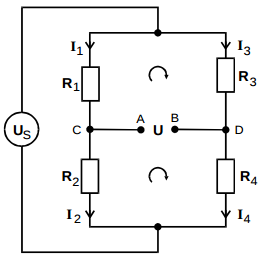
\includegraphics[width=0.5\textwidth]{V3021.png}
  \caption{Schaltplan der allgemeinen Brückenschaltung. \cite{anleitung}}
  \label{fig:V3021}
\end{figure}
In Abbildung \ref{fig:V3021} ist der Aufbau der allgemeinen
Brückenschaltung zu sehen. An den Punkten A und B wird die Brückenspannung abgegriffen.
Sie wird durch das Verhältnis der eingebrachten Widerstände $R_1$ und $R_4$
bestimmt.
Wenn die Abgleichbedingung
\begin{equation}
    R_1 R_4 = R_2 R_3
    \label{eqn:abgleich}
\end{equation}
gegeben ist, ist eine Nullspannung erreicht. Für komplexe Widerstände folgt:
\begin{equation}
    Z = X + \mathup{i}Y.
\end{equation}
mit dem Wirkwiderstand X und dem Blindwiderstand Y. Die komplexen
Wechselstromwiderstände von einer idealen Kapazität $C$ und einer idealen
Induktivität $L$ sind, in Abhängigkeit von der Frequenz $\omega$, folgendermaßen
definiert:
\begin{equation}
    Z_C = -\frac{\mathup{i}}{\omega C} \quad \mathup{und} \quad Z_L = \mathup{i} \omega L.
    \label{eqn:impedanzen}
\end{equation}
Zwei komplexe Zahlen sind nur dann gleich, wenn die Real- und die Imaginärteile
dieser gleich sind. Für komplexe Widerstände ergibt sich aus Gleichung
\eqref{eqn:abgleich} die Abgleichbedingung
\begin{equation}
    \label{eqn:abgleich_komplex}
    Z_1 Z_4 = Z_2 Z_3.
\end{equation}
Damit folgt
\begin{align}
    \label{eqn:abgleich_komplex_1}
    X_1 X_4 - Y_1 Y_4 &= X_2 X_3 - Y_2 Y_3 \\
    \shortintertext{und}
    \label{eqn:abgleich_komplex_2}
    X_1 Y_4 + X_4 Y_1 &= X_2 Y_3 + X_3 Y_2.
\end{align}
\newpage
\subsection{Die Wheatstonesche Brücke}
\begin{figure}[htb]
  \centering
  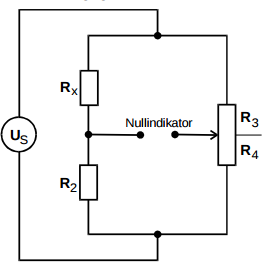
\includegraphics[width=0.5\textwidth]{V3022.png}
  \caption{Schaltplan der Wheatstoneschen Brücke. \cite{anleitung}}
  \label{fig:V3022}
\end{figure}
In Abbildung \ref{fig:V3022} zu sehen ist die Wheatstonesche Brückenschaltung.
Sie wird genutzt um einen unbekannten ohmschen Widerstand $R_x$ zu bestimmen.
Bei einer Wheatstoneschen Brückenschaltung kann mit Gleich- und
Wechselstrom gearbeitet werden. Durch die Abgleichbeziehung ergibt sich,
dass durch die Änderung des Verhältnisses von $R_3$ und $R_4$, die
Brückenspannung auf 0 gebracht wird. Damit folgt
\begin{equation}
    \label{eqn:wheatstone}
    R_{\mathup{x}} = R_2 \frac{R_3}{R_4}
\end{equation}
\newpage
\subsection{Die Kapazitätsmessbrücke}
\begin{figure}[htb]
  \centering
  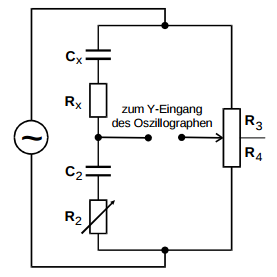
\includegraphics[width=0.5\textwidth]{V3023.png}
  \caption{Schaltplan der Kapazitätsmessbrücke. \cite{anleitung}}
  \label{fig:V3023}
\end{figure}
In Abbildung \ref{fig:V3023} zu sehen ist die Brückenschaltung für die
Kapazitätsmessbrücke. Nun wird der unbekannte Widerstand $R_x$ durch einen
Kondensator $C_x$ ersetzt. Da der Kondensator allerdings auch verlustbehaftet
ist, ist im Schaltbild \ref{fig:V3023} ein fiktiver Widerstand $R_x$
berücksichtigt. Aus den beiden vorherigen Ausgleichsbedingungen folgt für
die Kapazitätsmessbrücke der Zusammenhang
\begin{align}
    \label{eqn:kapazitätsmessbrücke_R}
    R_{\mathup{x}} &= R_2 \frac{R_3}{R_4} \\
    \shortintertext{und}
    \label{eqn:kapazitätsmessbrücke_C}
    C_{\mathup{x}} &= C_2 \frac{R_4}{R_3}.
\end{align}

\newpage
\subsection{Die Induktivitätsmessbrücke}
\begin{figure}[htb]
  \centering
  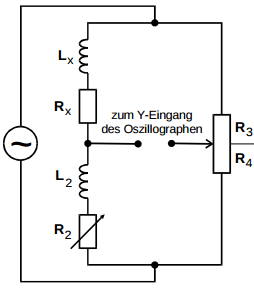
\includegraphics[width=0.5\textwidth]{V3024.png}
  \caption{Schaltplan der Induktivitätsmessbrücke. \cite{anleitung}}
  \label{fig:V3024}
\end{figure}
In Abbildung \ref{fig:V3024} zu sehen ist die Brückenschaltung für die
Induktivitätsmessbrücke. Induktivitäten werden dabei analog wie bei der
Kapazitätsmessbrücke bestimmt, mit dem Unterschied, dass die Kapazitäten
durch Induktivitäten ersetzt werden. Dabei folgen aus den Abgleichbedingungen
folgende Zusammenhänge
\begin{align}
    \label{eqn:induktivitätsmessbrücke_R}
    R_{\mathup{x}} &= R_2 \frac{R_3}{R_4} \\
    \label{eqn:induktivitätsmessbrücke_L}
    L_{\mathup{x}} &= L_2 \frac{R_3}{R_4}.
\end{align}
\newpage
\subsection{Die Maxwell-Brücke}
\begin{figure}[htb]
  \centering
  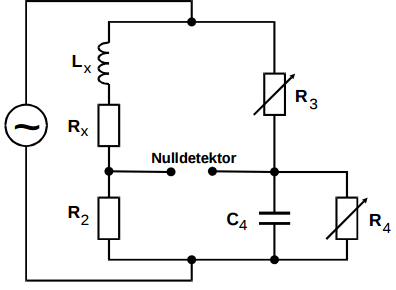
\includegraphics[width=0.5\textwidth]{V3025.png}
  \caption{Schaltplan der Maxwell-Brücke. \cite{anleitung}}
  \label{fig:V3025}
\end{figure}
In Abbildung \ref{fig:V3025} zu sehen ist die Brückenschaltung für die
Maxwell-Brücke. Hier wird auf die Induktivität $L_2$, welche bei der Induktivitätsmessbrücke
noch verwendet wurde, verzichtet. Stattdessen wird mit einem Kondensator $C_4$
gearbeitet. Aus den Abgleichbedingungen folgen dann die Beziehungen
\begin{align}
    \label{eqn:maxwell_R}
    R_{\mathup{x}} &= \frac{R_2 R_3}{R_4} \\
    \shortintertext{und}
    \label{eqn:maxwell_L}
    L_{\mathup{x}} &= R_2 R_3 C_4.
\end{align}

\newpage
\subsection{Die Wien-Robinson-Brücke}
\begin{figure}[htb]
  \centering
  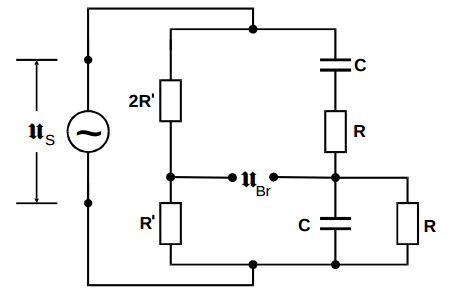
\includegraphics[width=0.5\textwidth]{V3026.png}
  \caption{Schaltplan der Wien-Robinson-Brücke. \cite{anleitung}}
  \label{fig:V3026}
\end{figure}
In Abbildung \ref{fig:V3026} zu sehen ist die Brückenschaltung für die
Wien-Robinson-Brücke. Nun werden keine unbekannten Induktivitäten, Widerstände
oder Kapazitäten mehr genutzt, sondern es wird die Frequenzabhängigkeit
untersucht. Die Wien-Robinson-Brücke fungiert als Sperrfilter. Ein Sperrfilter
filtert eine bestimmte Frequenz einer Spannungsquelle vollständig aus dem
Spektrum heraus. Das Verhältnis zwischen Brückenspannung $U_\mathup{Br}$ und Quellspannung
$U_\mathup{S}$ kann man mit Hilfe der Kirchhoffschen Regeln \eqref{eqn:Knotenregel} als
\begin{equation}
    \label{eqn:wien_robinson_1}
    \left|\frac{U_\mathup{Br}}{U_\mathup{S}}\right|^2 = \frac{\left(\omega^2 R^2 C^2 - 1\right)^2}{9\left(\left(1 - \omega^2 R^2 C^2\right)^2 + 9 \omega^2 R^2 C^2\right)}.
\end{equation}
ausdrücken.
\newpage
\section{Durchführung}
\label{sec:durchführung}
\subsection{Widerstandsmessung}
Als erstes wird in dem Versuch mit einer Wheatstoneschen Brücke, wie in
Abbildung \ref{fig:V3022} dargestellt, gearbeitet. Sie ist an einer
Wechselstromspannungsquelle angeschlossen. Zu bestimmen ist der Widerstand $R_x$.
Dieser ist unbekannt. Um $R_x$ zu bestimmen, wird das am Potentiometer
regelbare Verhältnis der beiden Widerstände $R_3$ und $R_4$ so eingestellt, dass
der Oszillograph eine Nullspaannung anzeigt. Diese Messung wird an zwei
verschiedenen unbekannten Widerständen $R_x$ durchgeführt, mit drei verschiedenen
$R_2$-Widerständen, um die Messgenauigkeit zu verbessern.
\subsection{Kapazitätsmessung}
Als nächstes wird eine Kapazitätsmessung durchgeführt. Dafür wird die Schaltung,
wie in \ref{fig:V3023} dargestellt, verändert. Wie auch schon bei der
Widerstandsmessung wird erneut die Nullspannung gesucht. Diese Messung wird
für einen weiteren idealen Kondensator wiederholt. Bei der nächsten Messung wird ein Kondensator
verwendet, der einen Wirkanteil in seinem Widerstand hat. Auch hier
wird eine Nullspannung gesucht. Dabei wird so abwechselnd variiert, bis ein
absolutes Minimum nahe Null gefunden wird. Dabei werden beide eingestellten
Widerstände notiert. Außerdem wird jede Messung mit drei verschiedenen
Kapazitäten $C_2$ durchgeführt.
\newpage
\subsection{Induktivitätsmessung}
Als nächstes wird eine Induktivitätsmessung durchgeführt. Dafür wird ein Aufbau.
wie in Abbildung \ref{fig:V3024} zu sehen, genutzt. Diese Messung
ist, vom Ablauf her, analog zu der Kapazitätsmessung. Um hier eine bessere
Messgenauigkeit zu gewährleisten wird die Messung mit drei verschiedenen
$L_2$-Induktivitäten durchgeführt.
Daraufhin wird mit einer Maxwell-Brücke, wie in Abbildung \ref{fig:V3025} zu
sehen, dieselbe Induktivität, wie bei der ersten Induktivitätsmessung,
bestimmt. Die Werte werden für $R_3$ und $R_4$ bestimmt und die Messung wird
für zwei weitere $R_2$-Widerstände wiederholt.

\subsection{Untersuchung der Frequenzanhängigkeit einer Wien-Robinson-Brücke}
Als letztes wird die Frequenzabhängigkeit einer Brückenschaltung untersucht.
Dafür nutzt man eine Wien-Robinson-Brücke, wie in Abbildung \ref{fig:V3026}
zu sehen. Der in der Schaltung enthaltene Wechselstromgenerator liefert eine
Quellspannung $U_\mathup{S}$. Diese Spannung hat eine variable bzw.
einstellbare Frequenz. Zur Messung wird dann die Brückenspannung $U_\mathup{Br}$ gegen die
Frequenz $f$ zwischen \SI{20}{\hertz} und \SI{20}{\kilo\hertz}
aufgenommen. Es werden für die Frequenz, $U_\mathup{S}$ und $U_\mathup{Br}$ je 37 Werte aufgenommen.
Dabei wird auf das Spannungsminimum von $U_\mathup{Br}$ besonders Wert gelegt, indem man
vorallem Spannungswerte zu den Frequenzen bestimmt, die nahe an dem
Spannungsminimum bei einer Frequenz von \SI{378}{\hertz} liegen.
\newpage

\section{Auswertung}
\label{sec:auswertung}
\subsection{Messwerte}
Bei den verschiedenen Versuchsabschnitten wurden die folgenden Werte Gemessen:
\begin{table}
  \centering
  \caption{a)Messwerte zur Wheatstoneschen Brücke.}
  \label{tab:messwerte1}
  \sisetup{table-format=3.0}
  \begin{tabular}{S[table-format=4.0] S[table-format=3.1] S[table-format=3.1] S[table-format=4.0] S S}
    \toprule
    \multicolumn{3}{c}{Widerstand 1 (Wert 11)} & \multicolumn{3}{c}{Widerstand 2 (Wert 12)}\\
    {$R_2 \,/\, \si{\ohm}$} & {$R_3 \,/\, \si{\ohm}$} & {$R_4 \,/\, \si{\ohm}$} & {$R_2 \,/\, \si{\ohm}$} & {$R_3 \,/\, \si{\ohm}$} & {$R_4 \,/\, \si{\ohm}$}\\
    \midrule
    332 & 596.0 & 404.0 & 332 & 540 & 460\\
    664 & 423.5 & 576.5 & 664 & 369 & 631\\
    1000 & 328.0 & 672.0 & 1000 & 280 & 720\\
    \bottomrule
  \end{tabular}
\end{table}
\begin{table}
  \centering
  \caption{b)Messwerte zur Kapazitätsmessbrücke.}
  \label{tab:messwerte2}
  \sisetup{table-format=3.0}
  \begin{tabular}{S S S S S[table-format=3.1] S[table-format=3.1]}
    \toprule
    \multicolumn{3}{c}{Kapazität 1 (Wert 1)} & \multicolumn{3}{c}{Kapazität 2 (Wert 3)}\\
    {$C_2 \,/\, \si{\nano\farad}$} & {$R_3 \,/\, \si{\ohm}$} & {$R_4 \,/\, \si{\ohm}$} & {$C_2 \,/\, \si{\nano\farad}$} & {$R_3 \,/\, \si{\ohm}$} & {$R_4 \,/\, \si{\ohm}$}\\
    \midrule
    399 & 376 & 624 & 399 & 486.5 & 513.5\\
    597 & 475 & 525 & 597 & 587.0 & 413.0\\
    994 & 600 & 400 & 994 & 702.0 & 298.0\\
    \bottomrule
  \end{tabular}
\end{table}
\begin{table}
  \centering
  \caption{b)Messwerte zur Kapazitätsmessbrücke.}
  \label{tab:messwerte3}
  \sisetup{table-format=3.1}
  \begin{tabular}{S[table-format=3.0] S S S}
    \toprule
    \multicolumn{4}{c}{RC Kombination (Wert 8)}\\
    {$C_2 \,/\, \si{\nano\farad}$} & {$R_2 \,/\, \si{\ohm}$} & {$R_3 \,/\, \si{\ohm}$} & {$R_4 \,/\, \si{\ohm}$}\\
    \midrule
    399 & 408.0 & 574.5 & 425.5\\
    597 & 267.5 & 670.0 & 330.0\\
    994 & 157.5 & 770.5 & 229.5\\
    \bottomrule
  \end{tabular}
\end{table}
\clearpage
\begin{table}
  \centering
  \caption{c)Messwerte zur Induktivitätsmessbrücke.}
  \label{tab:messwerte4}
  \sisetup{table-format=3.1}
  \begin{tabular}{S[table-format=2.1] S S S}
    \toprule
    \multicolumn{4}{c}{LR Kombination (Wert 18)}\\
    {$L_2 \,/\, \si{\milli\henry}$} & {$R_2 \,/\, \si{\ohm}$} & {$R_3 \,/\, \si{\ohm}$} & {$R_4 \,/\, \si{\ohm}$}\\
    \midrule
    14.6 & 104.5 & 772.0 & 228.0\\
    20.1 & 139.0 & 713.0 & 287.0\\
    27.5 & 196.0 & 645.5 & 354.5\\
    \bottomrule
  \end{tabular}
\end{table}
\begin{table}
  \centering
  \caption{d)Messwerte zur Maxwell-Brücke (Wert 18).}
  \label{tab:messwerte5}
  \sisetup{table-format=3.1}
  \begin{tabular}{S[table-format=4.0] S S}
    \toprule
    {$R_2 \,/\, \si{\ohm}$} & {$R_3 \,/\, \si{\ohm}$} & {$R_4 \,/\, \si{\ohm}$}\\
    \midrule
    1000 & 48.0 & 138.5\\
    664 & 73.5 & 138.0\\
    332 & 148.5 & 138.0\\
    \bottomrule
  \end{tabular}
\end{table}

Für den Aufbau der Wien-Robinson-Brücke wurden die folgenden Bauteile verwendet:
\begin{align}
  R' &= \SI{332}{\ohm} \\
  R &= \SI{1}{\kilo\ohm} \\
  C &= \SI{421}{\nano\farad} \; \left( \text{Die zuvor bestimmte Kapazität Wert 3} \right)
\end{align}
Damit wurden dann die in Tabelle \ref{tab:messwerte6} stehenden Werte gemessen.
\begin{table}
  \centering
  \caption{Messwerte zur Wien-Robinson-Brücke.}
  \label{tab:messwerte6}
  \sisetup{table-format=1.3}
  \begin{tabular}{S[table-format=5.0] S S[table-format=1.4]}
    \toprule
    {$f \,/\, \si{\hertz}$} & {$U_\mathup{S} \,/\, \si{\volt}$} & {$U_\mathup{Br} \,/\, \si{\volt}$}\\
    \midrule
    300 & 2.94 & 0.384\\
    305 & 2.94 & 0.364\\
    310 & 2.94 & 0.336\\
    315 & 2.94 & 0.312\\
    320 & 2.94 & 0.290\\
    325 & 2.94 & 0.266\\
    330 & 2.925 & 0.240\\
    335 & 2.925 & 0.208\\
    340 & 2.925 & 0.188\\
    345 & 2.925 & 0.156\\
    350 & 2.925 & 0.131\\
    355 & 2.925 & 0.102\\
    360 & 2.94 & 0.0808\\
    365 & 2.94 & 0.064\\
    370 & 2.925 & 0.04\\
    375 & 2.925 & 0.0176\\
    378 & 2.925 & 0.0152\\
    385 & 2.86 & 0.033\\
    390 & 2.9 & 0.067\\
    395 & 2.9 & 0.085\\
    400 & 2.95 & 0.11\\
    405 & 2.95 & 0.127\\
    410 & 2.94 & 0.158\\
    415 & 2.95 & 0.166\\
    420 & 2.95 & 0.194\\
    430 & 2.85 & 0.238\\
    440 & 2.85 & 0.270\\
    450 & 2.86 & 0.296\\
    500 & 2.86 & 0.496\\
    600 & 2.85 & 0.776\\
    1000 & 2.8 & 1.46\\
    1500 & 2.725 & 1.86\\
    2000 & 2.79 & 2.06\\
    5000 & 2.725 & 2.3\\
    10000 & 2.725 & 2.3\\
    15000 & 2.74 & 2.26\\
    20000 & 2.76 & 2.26\\
    \bottomrule
  \end{tabular}
\end{table}
\newpage
\subsection{a)Berechnung von zwei unbekannten Widerständen (Wheatstone)}
Zur Berechnung der zwei unbekannten Widerstände wird Formel \eqref{eqn:wheatstone}
verwendet. Aus den jeweils drei Messungen folgen dann entsprechend sechs Ergebnisse:
\begin{table}
  \centering
  \label{tab:ergebnisse1}
  \begin{tabular}{c c}
    \toprule
    Widerstand 1 (Wert 11) & Widerstand 2 (Wert 12)\\
    \midrule
    \num{490} & \num{390}\\
    \num{488} & \num{388}\\
    \num{488} & \num{389}\\
    \bottomrule
  \end{tabular}
\end{table}
\\
Durch Mitteln ergibt sich für den ersten Widerstand (Wert 11)
\begin{equation}
  R_\text{Wert 11} = \SI{488.6(6)}{\ohm}.
\end{equation}
Für den zweiten Widerstand (Wert 12) ergibt sich
\begin{equation}
  R_\text{Wert 12} = \SI{389.0(6)}{\ohm}.
\end{equation}

\subsection{b)Berechnung von zwei Kapazitäten sowie einer RC Kombination}
Zur Berechnung der drei Kapazitäten wird Formel \eqref{eqn:kapazitätsmessbrücke_C}
verwendet, während für den Widerstand der RC Kombination Formel \eqref{eqn:kapazitätsmessbrücke_R} verwendet wird.
Die Ergebnisse der einzelnen Messungen sind:
\begin{table}
  \centering
  \label{tab:ergebnisse2.1}
  \begin{tabular}{c c}
    \toprule
    Kapazität 1 (Wert 1)/ $\si{\nano\farad}$ & Kapazität 2 (Wert 3)/ $\si{\nano\farad}$\\
    \midrule
    \num{662} & \num{421}\\
    \num{660} & \num{420}\\
    \num{663} & \num{422}\\
    \bottomrule
  \end{tabular}
\end{table}
\begin{table}
  \centering
  \label{tab:ergebnisse2.2}
  \begin{tabular}{c c}
    \toprule
    Kapazität 3 (Wert 8)/ $\si{\nano\farad}$ & Widerstand 3 (Wert 8)/ $\si{\ohm}$\\
    \midrule
    \num{296} & \num{551}\\
    \num{294} & \num{543}\\
    \num{296} & \num{529}\\
    \bottomrule
  \end{tabular}
\end{table}
\\
Durch Mitteln ergibt sich für die erste Kapazität (Wert 1)
\begin{equation}
  C_\text{Wert 1} = \SI{661.6(9)}{\nano\farad}.
\end{equation}
Für die zweite Kapazität (Wert 3) ergibt sich
\begin{equation}
  C_\text{Wert 3} = \SI{421.0(6)}{\nano\farad}.
\end{equation}
\\
Als Kapazität und Widerstand der RC Kombination (Wert 8) ergeben sich
\begin{align}
  C_\text{Wert 8} &= \SI{295.2(6)}{\nano\farad}\\
  R_\text{Wert 8} &= \SI{541(6)}{\ohm}
\end{align}

\subsection{c)+d)Berechnung der Induktivität einer Spule sowie ihres Verlustwiderstands}
Zunächst wird die Induktivität und der Verlustwiderstand der Spule (Wert 18), mit den
in Tabelle \ref{tab:messwerte4} stehenden Werten und den Formeln \eqref{eqn:induktivitätsmessbrücke_L}
sowie \eqref{eqn:induktivitätsmessbrücke_R}, berechnet. Die Ergebnisse davon sind:
\begin{table}
  \centering
  \label{tab:ergebnisse3}
  \begin{tabular}{c c}
    \toprule
    Induktivität (Wert 18)/ $\si{\milli\henry}$ & Verlustwiderstand (Wert 18)/ $\si{\ohm}$\\
    \midrule
    \num{49.4} & \num{354}\\
    \num{49.9} & \num{345}\\
    \num{50.1} & \num{357}\\
    \bottomrule
  \end{tabular}
\end{table}
\\
Schließlich folgen für die Induktivität und den Verlustwiderstand diese gemittelten
Ergebnisse:
\begin{align}
  L_\text{Wert 18} &= \SI{49.8(2)}{\milli\henry}\\
  R_\text{Wert 18} &= \SI{352(3)}{\ohm}
\end{align}
\\
Nun werden die selben Größen erneut, mit den Messwerten aus Tabelle \ref{tab:messwerte5}
und den Formeln \eqref{eqn:maxwell_L} und \eqref{eqn:maxwell_R}, berechnet.
Die hierbei verwendete Kapazität $C_4$ beträgt $\SI{994}{\nano\farad}$.
\newpage
Daraus folgen diese Ergebnisse:
\begin{table}
  \centering
  \label{tab:ergebnisse4}
  \begin{tabular}{c c}
    \toprule
    Induktivität (Wert 18)/ $\si{\milli\henry}$ & Verlustwiderstand (Wert 18)/ $\si{\ohm}$\\
    \midrule
    \num{47.7} & \num{347}\\
    \num{48.5} & \num{354}\\
    \num{49.0} & \num{357}\\
    \bottomrule
  \end{tabular}
\end{table}
\\
Gemittelt ergeben sich dann folgende Werte für die Induktivität und den Widerstand:
\begin{align}
  L_\text{Wert 18} &= \SI{48.4(4)}{\milli\henry}\\
  R_\text{Wert 18} &= \SI{352(3)}{\ohm}
\end{align}

\subsection{e)Frequenzabhängikeit der Wien-Robinson-Brücke und f)Berechnung des Klirrfaktors des Generators}
Zuerst soll der Quotient aus der Brückenspannung und der Quellspannung $\left( \frac{U_\mathup{Br}}{U_\mathup{S}} \right)$
gegen das Verhältnis aus eingestellter Frequenz $\nu$ und der kritischen Frequenz $\nu_0$, beim
Minimalwert der Brückenspannung, halblogarithmisch aufgetragen werden.
Zu beachten ist dabei, dass die Werte von $U_\mathup{Br}$ in der Tabelle die Peak to Peak Messwerte sind.
Für den Graphen werden diese halbiert und nach
\begin{equation}
  U_{eff} = \frac{\hat{U}}{\sqrt{2}}
  \label{eqn:effektivspannung}
\end{equation}
die Effektivspannung ausgerechnet.
\\
\\
Aus $R = \SI{1}{\kilo\ohm}$ und $C = \SI{421}{\nano\farad}$ folgt nach
\begin{equation}
  \omega_0 = \frac{1}{R C}
  \label{eqn:omega0}
\end{equation}
eine kritische Kreisfrequenz von $\omega_0 = \SI{2375}{\per\second}$ und dem entsprechend
eine kritische Frequenz von $\nu_0 = \SI{378}{\hertz}$.
\\
\\
Durch einsetzen von \eqref{eqn:omega0} in Formel \eqref{eqn:wien_robinson_1}
ergibt sich
\begin{equation}
  \left|\frac{U_\mathup{Br}}{U_\mathup{S}}\right| = \sqrt{\frac{\left(\Omega^2 - 1\right)^2}{9\left(\left(1 - \Omega^2 \right)^2 + 9 \Omega^2 \right)}} \;\;\;\;\;\; \text{mit} \;\; \Omega = \frac{\nu}{\nu_0}.
  \label{eqn:wien_robinson_2}
\end{equation}
Diese Funktion wird ebenfalls in den Graphen eingezeichnet.

\begin{figure}
  \centering
  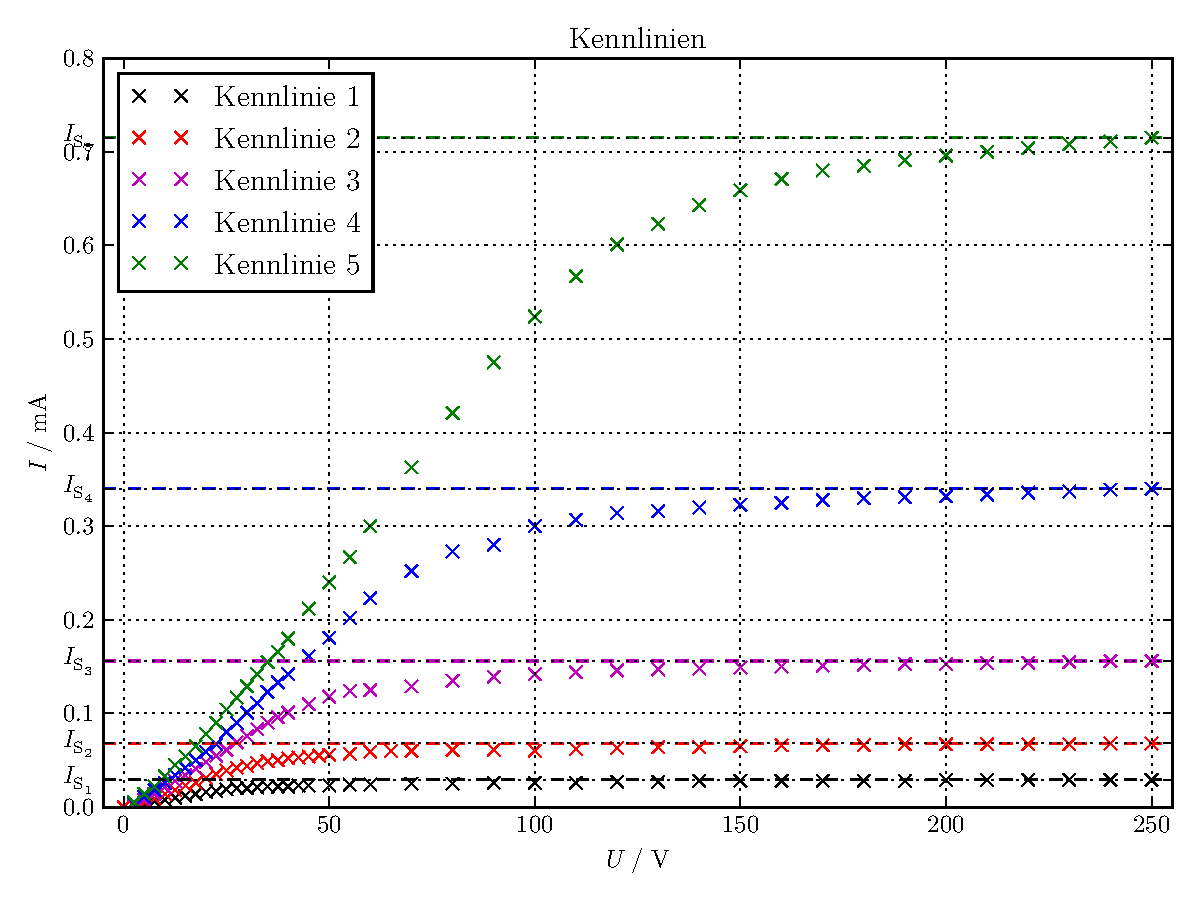
\includegraphics[width=\textwidth]{Plot.pdf}
  \caption{Frequenzabhängigkeit der Brückenspannung bei der Wien-Robinson-Brücke}
  \label{fig:plot}
\end{figure}

\begin{table}
  \centering
  \caption{Im Plot verwendete Werte.}
  \label{tab:messwerte6}
  \sisetup{table-format=1.4}
  \begin{tabular}{S S[table-format=2.3]}
    \toprule
    {$\frac{U_\mathup{Br_{eff}}}{U_\mathup{S}}$} & {$\frac{\nu}{\nu_0}$}\\
    \midrule
    0.0462 & 0.794\\
    0.0438 & 0.807\\
    0.0404 & 0.82\\
    0.0375 & 0.833\\
    0.0349 & 0.847\\
    0.032 & 0.86\\
    0.029 & 0.873\\
    0.0251 & 0.886\\
    0.0227 & 0.899\\
    0.0189 & 0.913\\
    0.0158 & 0.926\\
    0.0123 & 0.939\\
    0.0097 & 0.952\\
    0.0077 & 0.966\\
    0.0048 & 0.979\\
    0.0021 & 0.992\\
    0.0018 & 1\\
    0.0041 & 1.019\\
    0.0082 & 1.032\\
    0.0104 & 1.045\\
    0.0132 & 1.058\\
    0.0152 & 1.071\\
    0.019 & 1.085\\
    0.0199 & 1.098\\
    0.0233 & 1.111\\
    0.0295 & 1.138\\
    0.0335 & 1.164\\
    0.0366 & 1.190\\
    0.0613 & 1.323\\
    0.0963 & 1.587\\
    0.1844 & 2.646\\
    0.2413 & 3.968\\
    0.261 & 5.291\\
    0.2984 & 13.228\\
    0.2984 & 26.455\\
    0.2916 & 39.683\\
    0.2895 & 52.91\\
    \bottomrule
  \end{tabular}
\end{table}
\clearpage
Wie zu sehen ist, ist die Brückenspannung bei $\nu_0$ nicht 0. Das liegt daran, dass
der Generator neben der Grundwelle auch noch eine Oberwelle erzeugt. Die Größe des
Anteils der Oberwelle wird durch den Klirrfaktor angegeben.
Er berechnet sich in diesem Fall nach:
\begin{equation}
  k = \frac{U_2}{U_1}.
  \label{eqn:klirr}
\end{equation}
Hierbei ist $U_1 = U_\mathup{S}$ bei $\nu_0$.
\\
\\
$U_2$ berechnet sich nach:
\begin{equation}
  U_2 = \frac{U_\mathup{Br_{eff}}\left( \nu_0 \right)}{\sqrt{\frac{(2^2-1)^2}{(9\cdot((1-2^2)^2+9\cdot2^2)))}}}
  \label{eqn:u2}
\end{equation}
Damit folgt für $U_2$, $U_1$ und k:
\begin{align}
  U_1 &= \SI{2.925}{\volt}\\
  U_2 &= \SI{0.036}{\volt}\\
  k &= \num{0.012}
\end{align}

\section{Diskussion}
\label{sec:diskussion}
Grundsäzlich kann gesagt werden, dass die verwendeten Methoden zur Bestimmung der
verschiedenen Widerstände, Kapazitäten und Induktivitäten sehr präzise Ergebnisse liefern.
Die gemessenen Werte bezüglich der Frequenzabhängigkeit der Wien-Robinson-Brücke
liegen relativ genau auf der Kurve der Vergleichsfunktion. Nur bei sehr großen Frequenzen
gibt es relativ große Abweichungen. Das Verhalten, dass die Wien-Robinson-Brücke
einen gewissen Frequenzbereich nicht durch lässt, lässt sich damit bestätigen.
Der Klirrfaktor des Generators scheint mit $\SI{1.2}{\percent}$ relativ klein zu sein.\\
\nocite{*}
\printbibliography

\end{document}
